\documentclass[10pt]{article}

\usepackage[T1]{fontenc}
\usepackage{geometry}
\usepackage{amsmath, amssymb, amsthm}
\usepackage{bm}
\usepackage{cancel}
\usepackage{xcolor}
\usepackage{graphicx}

\title{Mechanics II - Exercises}
\author{Satvik Saha}
\date{}

\geometry{a4paper, margin=1in}
\setlength\parindent{0pt}
\renewcommand{\labelenumi}{(\alph{enumi})}
\renewcommand\CancelColor{\color{red}}
% \renewcommand\qedsymbol{$\blacksquare$}
\let\vec\boldsymbol
\newcommand{\uveci}{{\bm{\hat{\textnormal{\bfseries\i}}}}}
\newcommand{\uvecj}{{\bm{\hat{\textnormal{\bfseries\j}}}}}
\newcommand{\uveck}{{\bm{\hat{\textnormal{\bfseries k}}}}}
\newcommand\norm[1]{\left\lVert#1\right\rVert}
\newcommand\grad[1]{\vec{\nabla}#1}
\newcommand\divg[1]{\vec{\nabla}\cdot#1}
\newcommand\curl[1]{\vec{\nabla}\times#1}
\newcommand\pp[2]{\frac{\partial #1}{\partial #2}}
\newcommand\dd[2]{\frac{d #1}{d #2}}

\renewcommand\v{\vec{v}}
\renewcommand\u{\vec{u}}
\renewcommand\a{\vec{a}}

\newcounter{prob}
\def\problem{\stepcounter{prob}\paragraph{Exercise \arabic{prob}}}
\def\solution{\paragraph{Solution}}
\setcounter{prob}{11}

\begin{document}
        \par\textbf{IISER Kolkata} \hfill \textbf{Exercises}
        \vspace{3pt}
        \hrule
        \vspace{3pt}
        \begin{center}
                \LARGE{\textbf{PH 2102 : Mechanics II}}
        \end{center}
        \vspace{3pt}
        \hrule
        \vspace{3pt}
        Satvik Saha, \texttt{19MS154}, Group E\hfill\today
        \vspace{20pt}

        \problem Use the continuity equation,
        \[
                \pp{\rho}{t} + \divg{\vec{j}} = 0,
        \]
        to show that the net charge coming into a fixed volume is equal to the change in charge content.

        \solution Let $V$ be an arbitrary fixed volume, with boundary $\partial V$. The current flowing through an elementary area $dS$
        is given by $\vec{j}\cdot \hat{\vec{n}}\:dS$, where $\hat{\vec{n}}$ is the unit normal to $dS$. Integrating this over
        the entire boundary gives us the net current flux,
        \[
                \Phi \;=\; \int_{\partial V} \vec{j}\cdot \hat{\vec{n}}\:dS.
        \]
        If $\hat{\vec{n}}$ is chosen to point outwards, this integral represents the rate at which charge exits the volume $V$ across its boundary.
        The negation of this likewise represents the rate of entry of charge into $V$.
        Since $\partial V$ is a closed boundary, we can use Gauss's Divergence Theorem to obtain
        \[
                \Phi \;=\; \int_{V} \divg{\vec{j}}\:dV.
        \]
        Applying the continuity equation, we have
        \[
                \Phi \;=\; -\int_{V} \pp{\rho}{t}\:dV \;=\; -\dd{}{t}\int_{V}\rho\:dV \;=\; -\dd{}{t}Q_{V}.
        \]
        We have interchanged the order of the integral and the derivative, and have used the fact that the integral of the charge density
        over a fixed volume is equal to the charge $Q_V$ enclosed by that volume.
        Thus, we arrive at the integral form of the continuity equation,
        \[
                \dd{}{t}Q_{V} \,+\, \int_{\partial V} \vec{j}\cdot \hat{\vec{n}}\:dS \;=\; 0.
        \]
        Thus, the rate at which charge flows into a fixed volume is precisely balanced by the rate of increase in charge content.

        \problem In the below illustration of Compton scattering, show that
        \[
                \lambda_2 - \lambda_1 = \frac{h}{m_e}(1 - \cos\theta).
        \]
        \begin{center}
                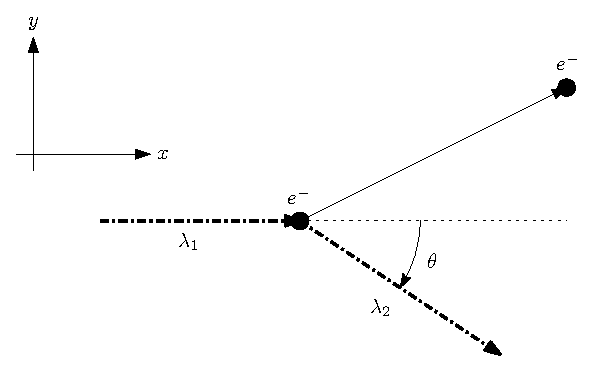
\includegraphics[scale=0.8]{./compton.eps}
        \end{center}

        \solution The four momentum of a particle is given by $p^\mu = (E, \vec{p})$. The conservation of energy and 3-momentum can thus
        be expressed together as the conservation of four momentum. Note that
        \[
                \norm{p^\mu}^2 = p^\mu\cdot p^\mu = E^2 - \norm{\vec{p}}^2 = m_0^2,
        \]
        where $m_0$ is the rest mass of the particle. Thus, we calculate the momenta before and after the collision.
        The incident wave initially has energy $h /\lambda_1$, which is also equal to its momentum along the $x$-axis, since
        it has rest mass zero and $E^2 = m_0^2 + p^2$. After the collision, it has energy $h /\lambda_2$ which is also equal to 
        its net momentum, directed at an angle $\theta$ to one side. Thus, its momenta along the $x$ and $y$ axes are $h\cos\theta /\lambda_2$
        and $h\sin\theta /\lambda_2$. The electron initially has energy $m_e$ (equal to its rest mass) and zero momentum as it was at rest.
        For the moment, let its four momentum after the collision be $p_e^\mu$. We thus write
        \[
                \underbrace{\left( \frac{h}{\lambda_1}, \frac{h}{\lambda_1}, 0, 0 \right)}_{p_1^\mu} \,+\, 
                        \underbrace{\left( m_0, 0, 0, 0 \right)}_{p_0^\mu} \;=\;
                        \underbrace{\left( \frac{h}{\lambda_2}, \frac{h}{\lambda_2}\cos\theta, \frac{h}{\lambda_2}\sin\theta, 0 \right)}_{p_2^\mu} 
                                \,+\, p_e^\mu.
        \]
        Isolating $p_e^\mu$ to one side and taking square norms, we have
        \begin{align*}
                \norm{p_1^\mu - p_2^\mu + p_0^\mu}^2 \;&=\; \norm{p_e^\mu}^2, \\
                \norm{p_1^\mu}^2 + \norm{p_2^\mu}^2 + \norm{p_0^\mu}^2 + 2p_1^\mu\cdot p_0^\mu - 2p_1^\mu\cdot p_2^\mu - 2p_2^\mu\cdot p_0^\mu
                        \;&=\; \norm{p_e^\mu}^2.
        \end{align*}
        Recall that $\norm{p_1^\mu}^2 = \norm{p_2^\mu}^2 = 0$, since the electromagnetic wave has zero rest mass. Furthermore, 
        $\norm{p_0^\mu}^2 = \norm{p_e^\mu}^2 = m_e^2$, so these cancel on both sides. We are thus left with
        \begin{align*}
                (p_1^\mu - p_2^\mu)\cdot p_0^\mu \;&=\; p_1^\mu \cdot p_2^\mu, \\
                \left(\frac{h}{\lambda_1} - \frac{h}{\lambda_2}\right)m_e \;&=\; \frac{h^2}{\lambda_1\lambda_2} - 
                        \frac{h^2}{\lambda_1\lambda_2}\cos\theta. \\
                \frac{\lambda_2 - \lambda_1}{\lambda_1\lambda_2}\, hm_e \;&=\; \frac{h^2}{\lambda_1\lambda_2}(1 - \cos\theta).
        \end{align*}
        Cancelling like terms, we obtain the desired expression,
        \[
                \lambda_2 - \lambda_1 = \frac{h}{m_e}(1 - \cos\theta).
        \]

        \problem A body of rest mass $m_0$ moving at speed $v$ collides with an identical body at rest. Thereafter, they stick together
        and move on. (a) Obtain the four-vector momentum of the final moving lump. (b) What is the rest mass of the resultant lump?

        \solution We simply calculate the four momenta of the the two bodies and add them together, since the conservation 
        of energy and 3-momenta guarantees that the four momentum of the system must be conserved.
        Supposing all motion is along the $x$ axis, the moving body initially has energy $E = \gamma m_0c^2$ and momentum $\gamma m_0 v$,
        where $\gamma = 1 /\sqrt{1 - v^2 / c^2}$. The stationary body initially has energy $m_0c^2$ and zero momentum, as it's at rest.
        Thus,
        \[
                p_f^\mu = \left(\gamma m_0c, \gamma m_0v, 0, 0\right) + \left(m_0c, 0, 0, 0\right) = \left((\gamma + 1)m_0c, \gamma m_0v, 0, 0\right).
                        \tag{a}
        \]
        We have already shown that the rest mass is simply given by the norm of $p^\mu$, up to a factor of $c$. Thus,
        \[
                \norm{p_f^\mu}^2 = (\gamma + 1)^2m_0^2c^2 - \gamma^2m_0^2 v^2 = m_0^2\left[\gamma^2c^2 + 2\gamma c^2 + c^2 - \gamma^2v^2\right].
        \]
        Now, $c^2 - v^2 = c^2 (1 - v^2 /c^2) = c^2 /\gamma^2$. Thus, our expression simplifies to
        \[
                \norm{p_f^\mu}^2 = m_0c^2\left[2 + 2\gamma\right] .
        \]
        Taking a square root and dividing by $c$, we obtain the final rest mass
        \[
                m_{0f} \;=\; m_0\sqrt{2 + 2\gamma} \;\geq\; 2m_0. \tag{b}
        \]

        \problem The earth and the sun are 8.3 light minutes apart. Ignore their relative motion and suppose that they are in the same intertial frame.
        Event A occurs at $t = 0$ on the earth, and event B occurs at $t = 2$ minutes on the sun. Find the time difference between the events
        according to an observer moving at speed $0.8\,c$ from the earth to the sun.

        \solution We set up our coordinate frames such that the $x$ axis extends from the earth to the sun. In the first frame,
        we observe a time separation $\Delta t = 2$ minutes and a spatial separation of $\Delta x = 8.3$ light minutes.
        Our moving frame has velocity $0.8\,c$ along the positive $x$ axis; its $\gamma$ factor is given by $1 /\sqrt{1 - 0.8^2} = 5 /3$.
        Using the Lorentz transformation $t' = \gamma(t - vx /c^2)$, we obtain the temporal separation in the moving frame
        \[
                \Delta t' = \gamma(\Delta t - v\Delta x /c) = \frac{5}{3} \left(2\text{ min} - (0.8)(8.3)\text{ min}\right) = -7.73\text{ minutes}.
        \]
        Thus, in the moving frame, the event on the sun occurs $7.33$ minutes \textit{before} that on the earth.
        This reversal of order suggests that the two events are not causally linked, which is evident from the fact that
        the events in the static frame occur too soon after another (2 minutes) for a signal to travel between them (at least 8.3 minutes).

        \problem An observer O who is on the $x$ axis of a frame records a flash of red light at $x_R = 1210$ m, and after $4\,\mu$s, 
        a flash of blue light at $x_B = 480$ m.
        \begin{enumerate}
                \item What is the velocity (relative to O) of an observer $O'$ moving along the $x$ axis who records the
                events as occurring at the same spatial point?
                \item Which flash occurs first according to $O'$ and what is the time interval between the two flashes as measured by $O'$?
        \end{enumerate}

        \solution Suppose the observer moves with speed $v$, and let this moving frame be recorded with primed coordinates.
        We use the Lorentz transformation $x' = \gamma(x - vt)$ to conclude that when $\Delta x' = 0$, we demand
        \[
                v = \frac{\Delta x}{\Delta t} = \frac{480 - 1210}{4\,\mu s} = -182.5\times 10^6 \text{ m/s} = -0.61\,c. \tag{a}
        \]
        Recall that since a signal can travel between the two events ($v < c$), the order of the events must be preserved between the frames,
        i.e.\ the red flash occurs first according to observer $O'$. In order to obtain the temporal separation, we use the invariance
        of the spacetime interval $c^2(\Delta t)^2 - (\Delta x)^2$, so
        \[
                (\Delta t')^2 = (\Delta t)^2 - (\Delta x)^2 /c^2 = 16\times 10^{-12} - 5.93\times 10^{-12} = 10.07\times 10^{-12} \text{ s}.
        \]
        Thus,
        \[
                \Delta t' = 3.17\,\mu s. \tag{b}
        \]

\end{document}
